\appendix
\chapter{Appendices}

\section{Appendix A: Use Case Diagrams}

\subsection{Inbound Property Inquiry Call --- Use Case Diagram}
\begin{figure}[H]
\centering
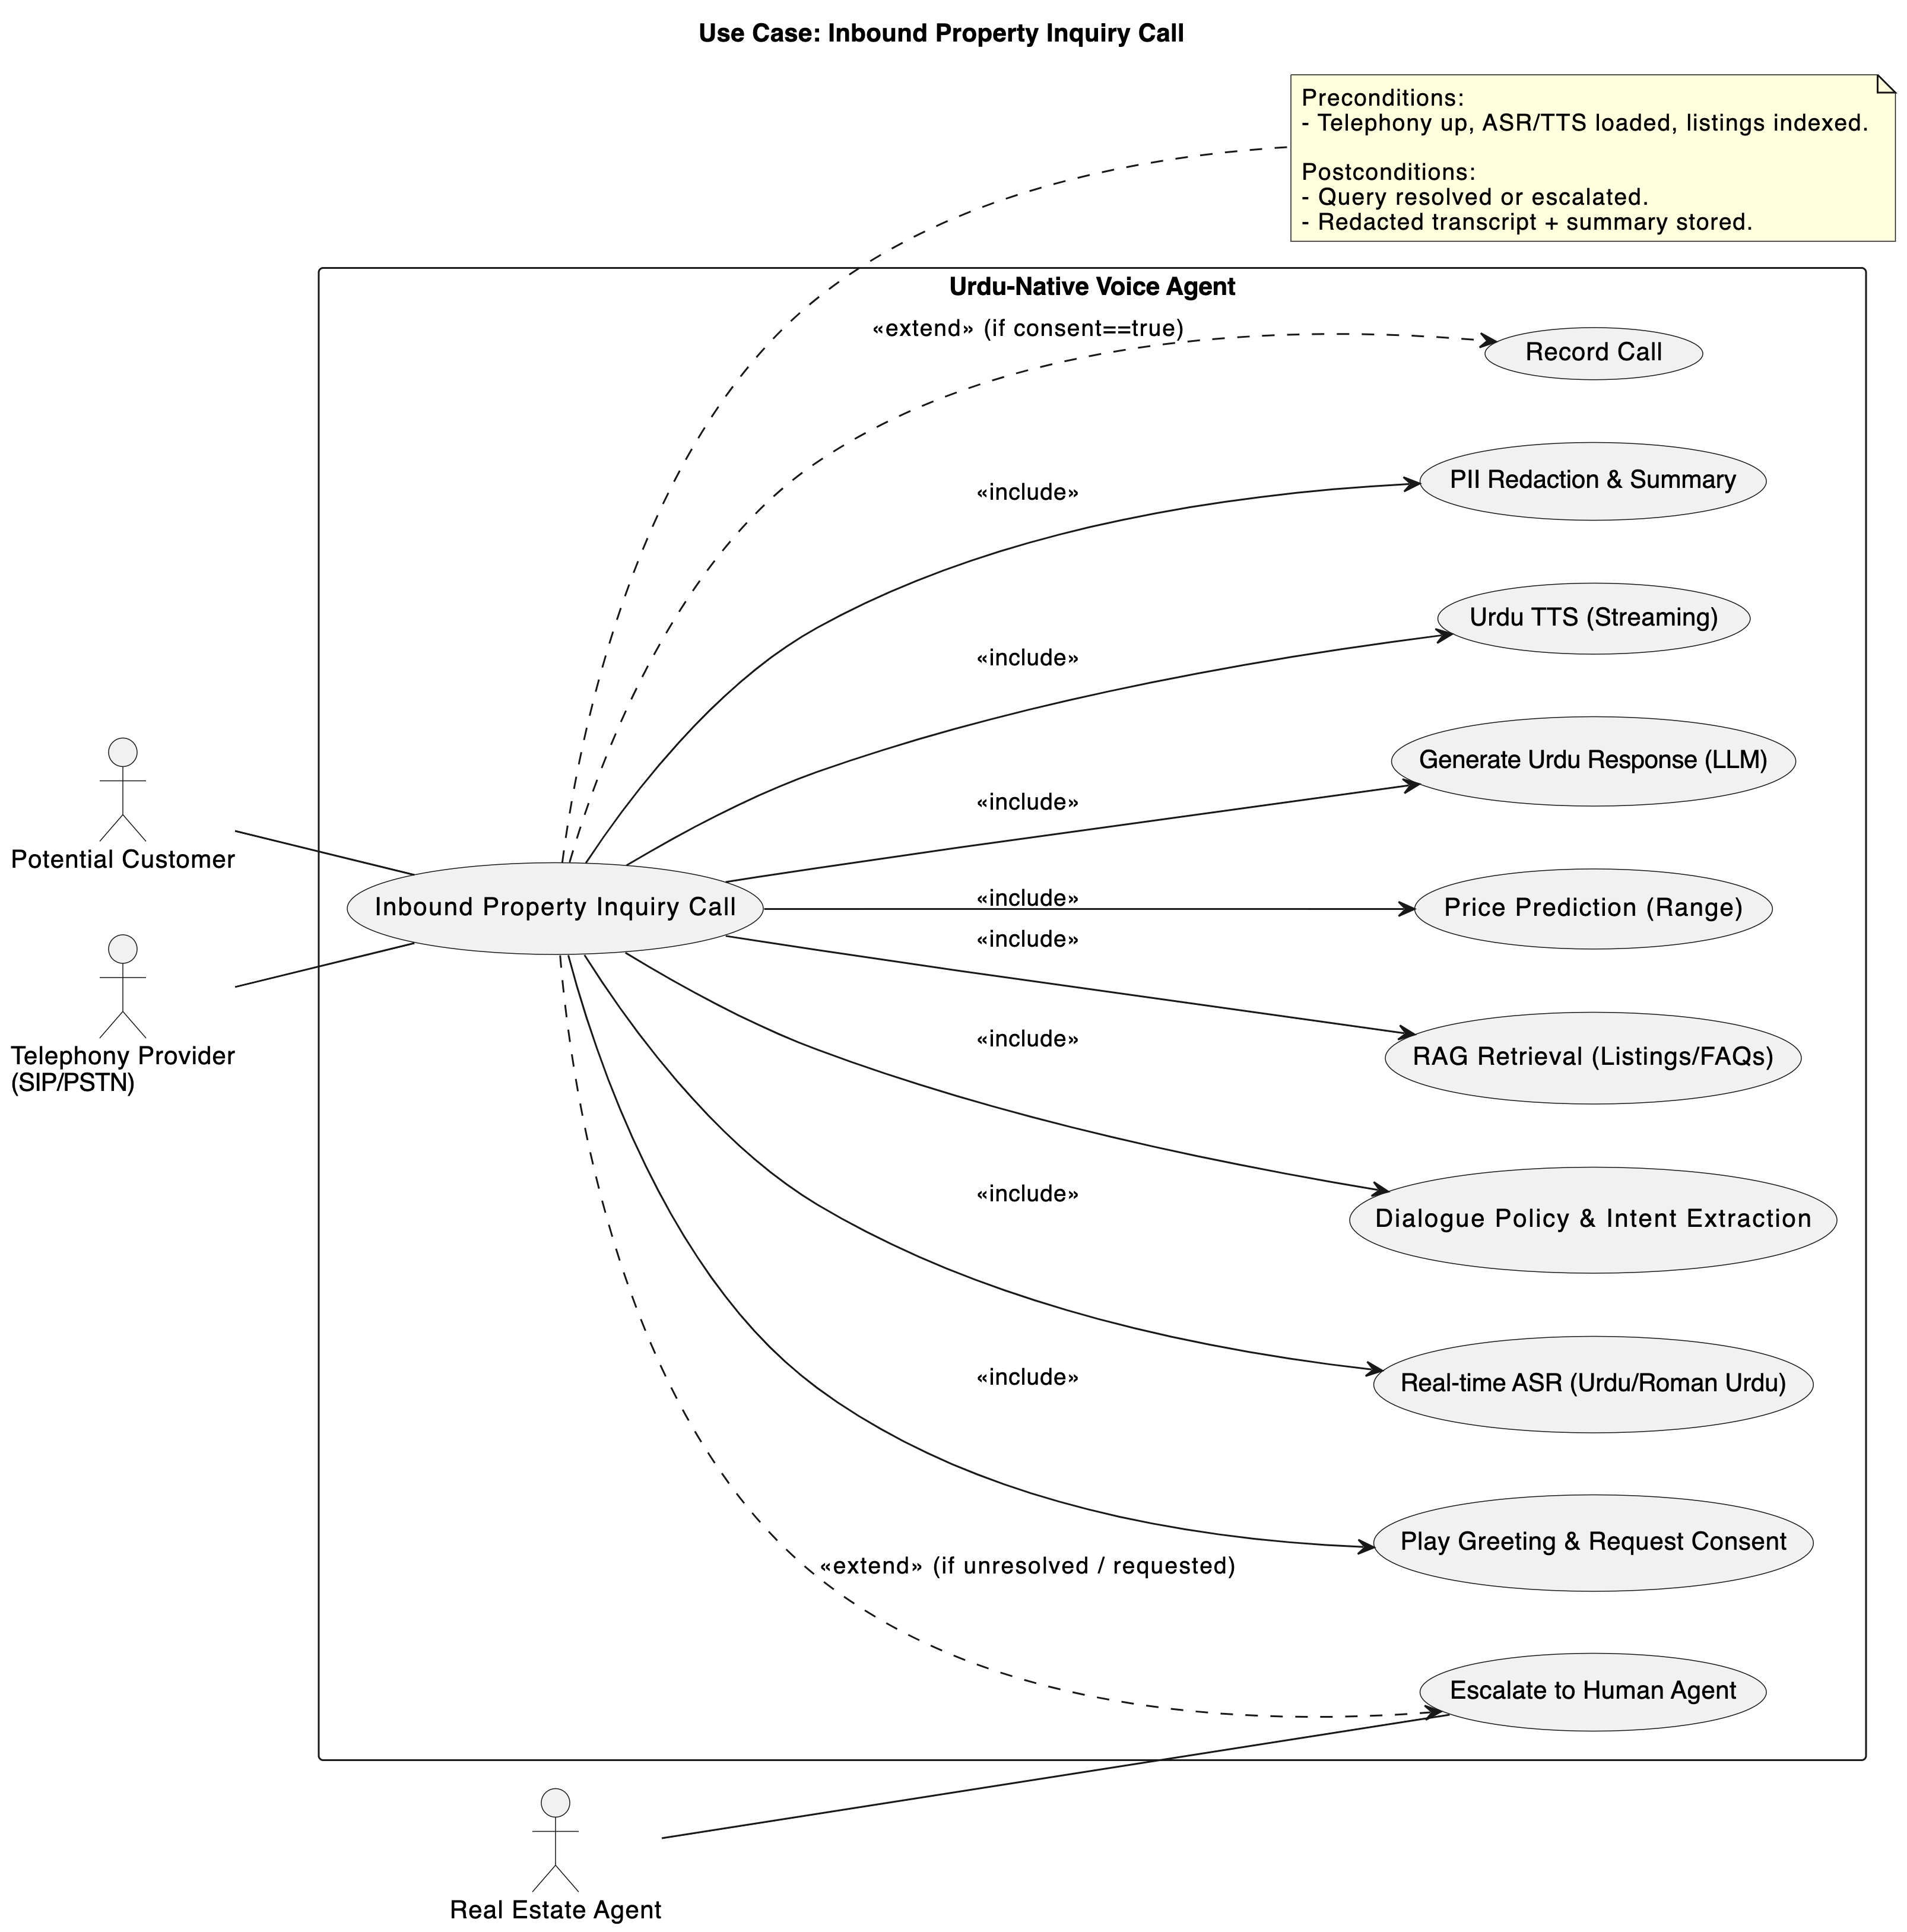
\includegraphics[width=\textwidth]{ThesisFigs/Use Case Diagram_FYP.drawio}
\caption{Inbound Property Inquiry Call --- Complete Use Case Diagram}
\label{fig:app-uc-inbound}
\end{figure}

\subsection{Outbound Lead Qualification Call --- Use Case Diagram}
\begin{figure}[H]
\centering
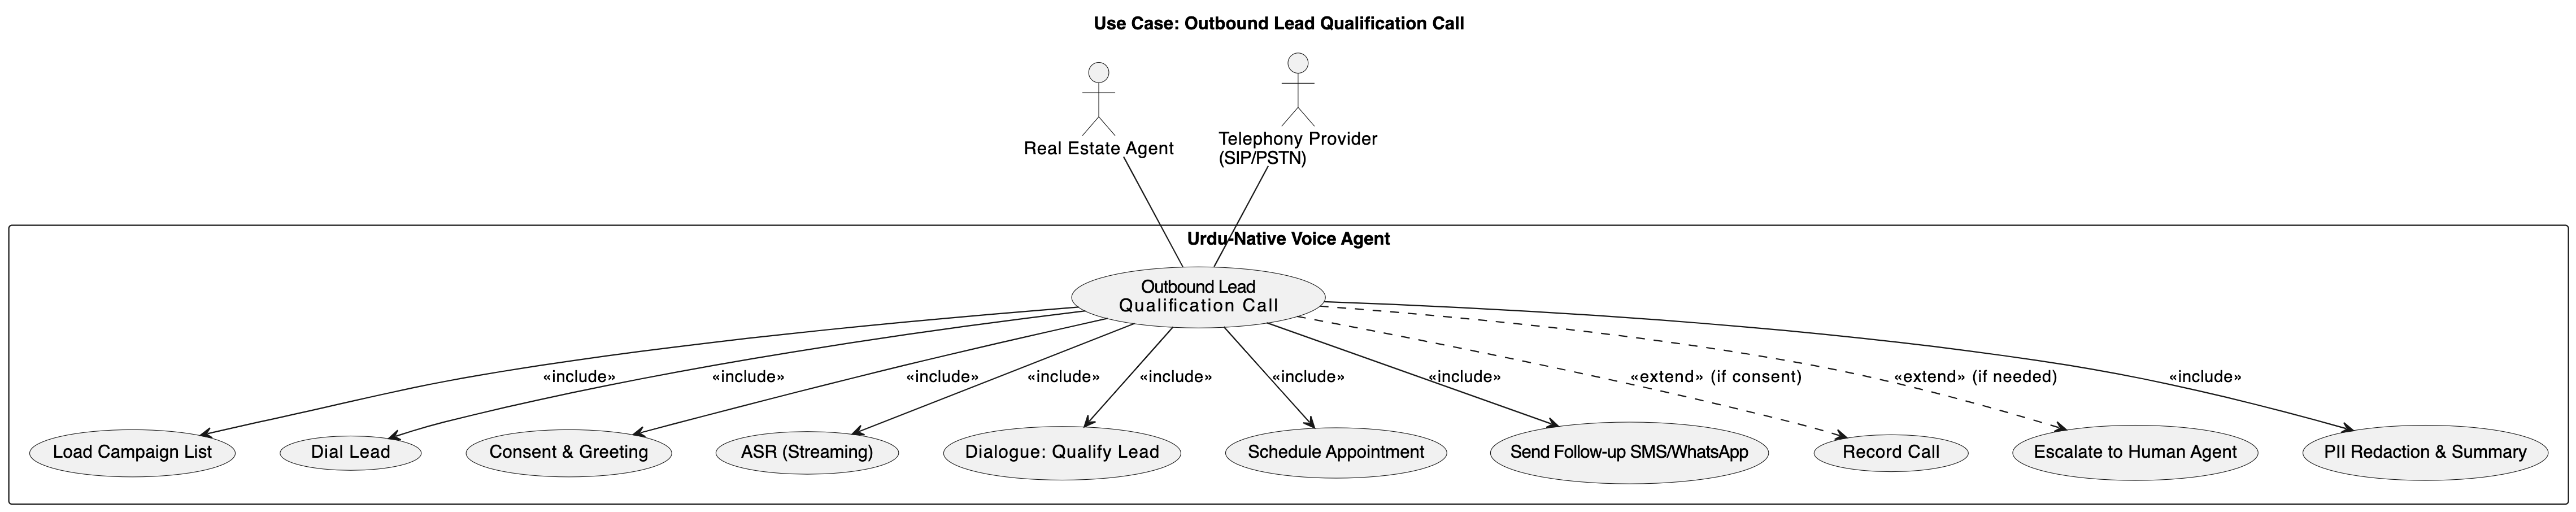
\includegraphics[width=0.9\textwidth]{ThesisFigs/Outbound Use case.drawio}
\caption{Outbound Lead Qualification Call --- Use Case Diagram}
\label{fig:app-uc-outbound}
\end{figure}

\subsection{Post-Call Analytics --- Use Case Diagram}
\begin{figure}[H]
\centering
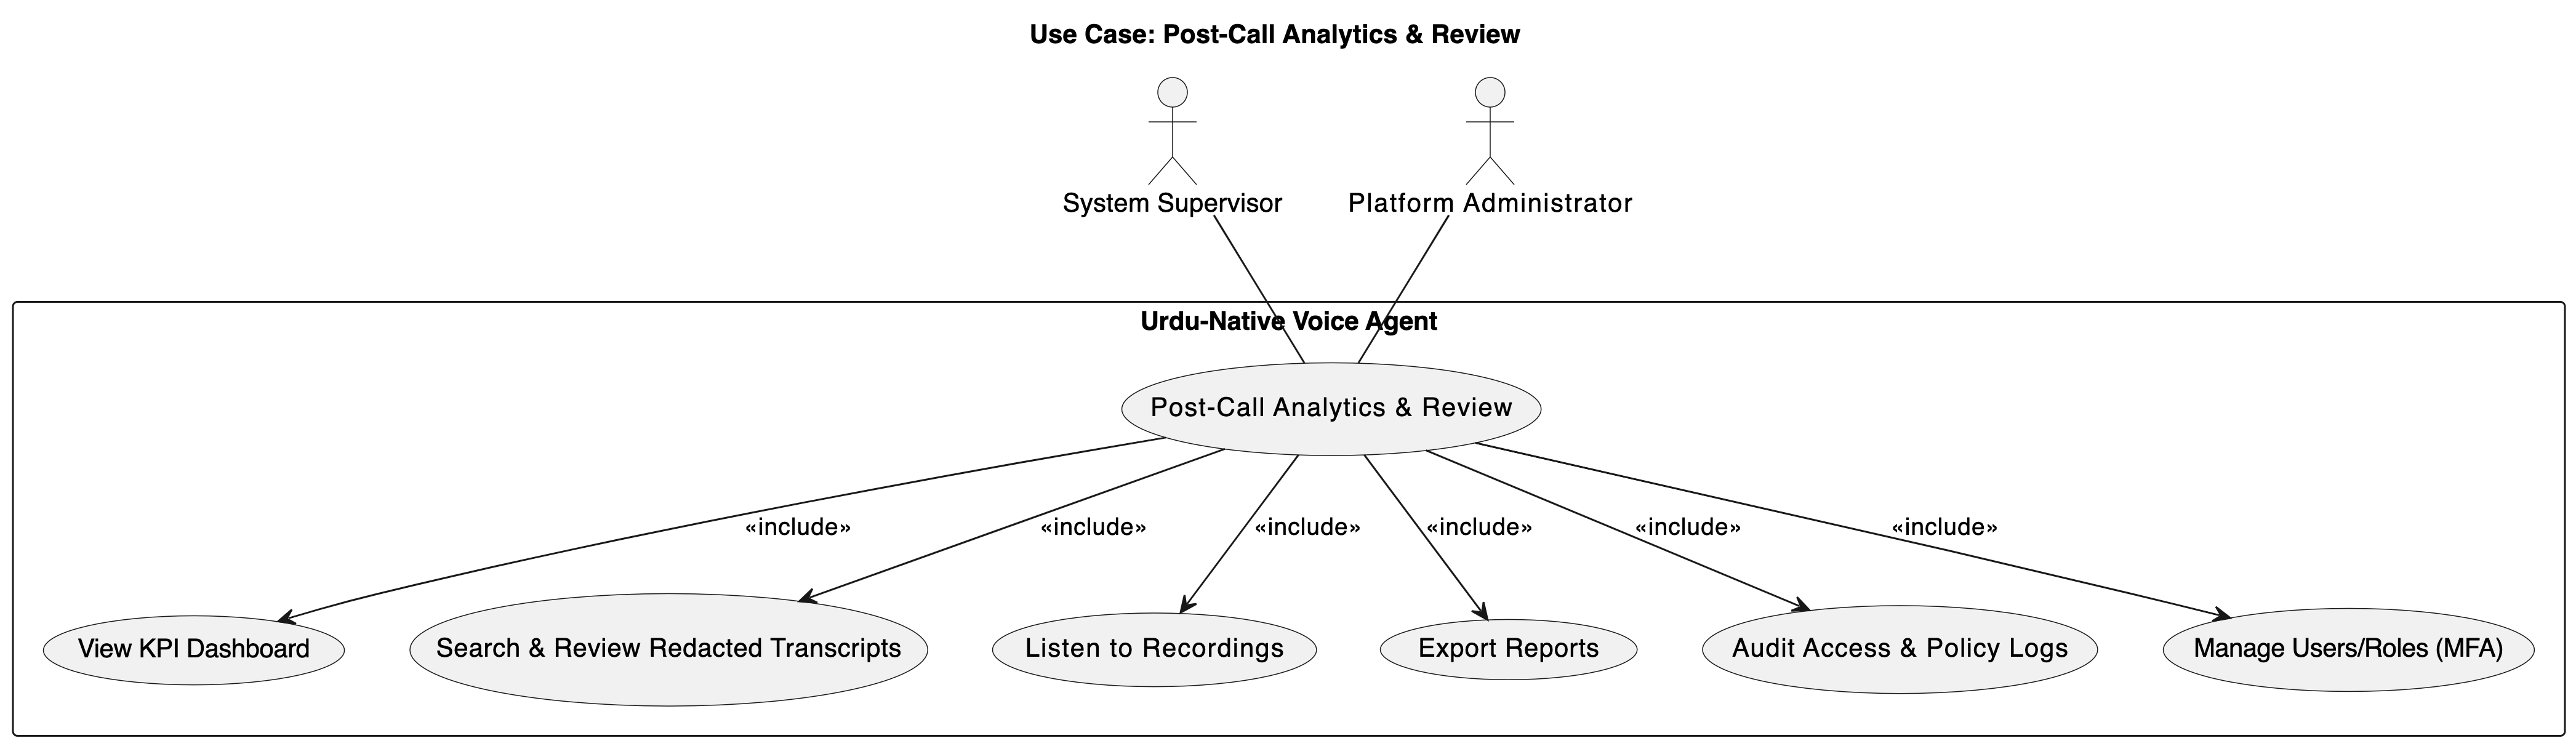
\includegraphics[width=0.9\textwidth]{ThesisFigs/PostCallAnalytics.drawio}
\caption{Post-Call Analytics and CRM Update --- Use Case Diagram}
\label{fig:app-uc-analytics}
\end{figure}

\subsection{Property Price Estimation --- Use Case Diagram}
\begin{figure}[H]
\centering
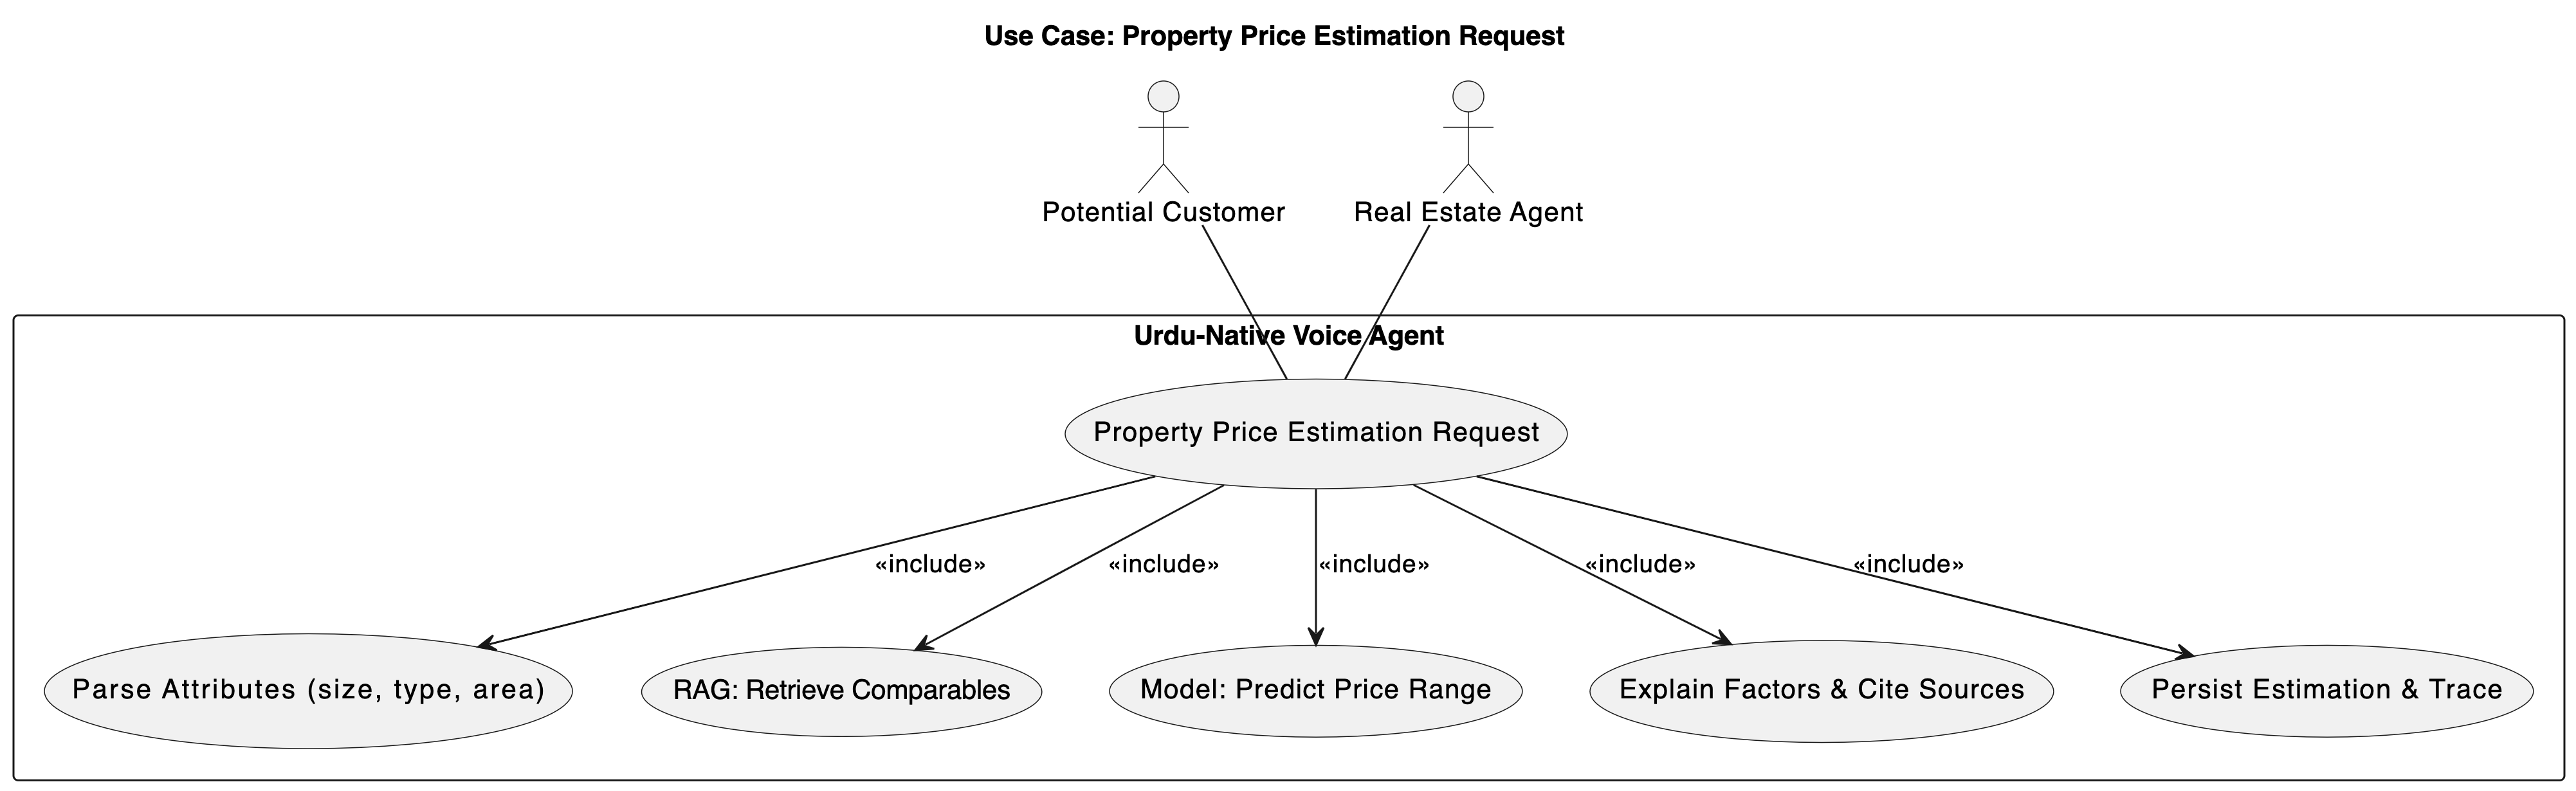
\includegraphics[width=0.85\textwidth]{ThesisFigs/PricePrediction}
\caption{Property Price Estimation --- Use Case Diagram}
\label{fig:app-uc-price}
\end{figure}

% ─── Additional Use Case Diagrams from Mid-Report ──────────────────────────
\subsection{System Admin Use Case}
\begin{figure}[H]
\centering
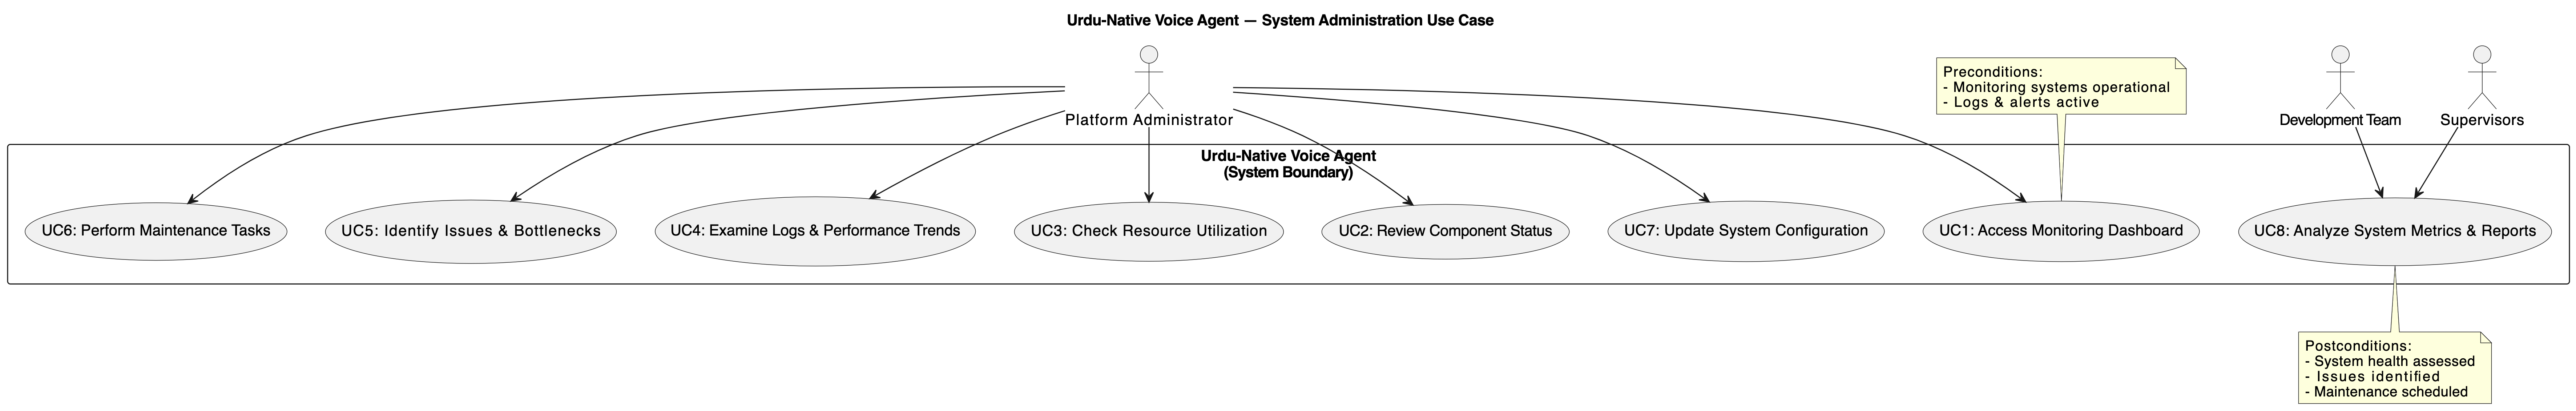
\includegraphics[width=\textwidth]{ThesisFigs/UC_ System Admin.drawio}
\caption{System Administrator Use Case Diagram}
\label{fig:app-uc-admin}
\end{figure}

\subsection{Data Management Use Case}
\begin{figure}[H]
\centering
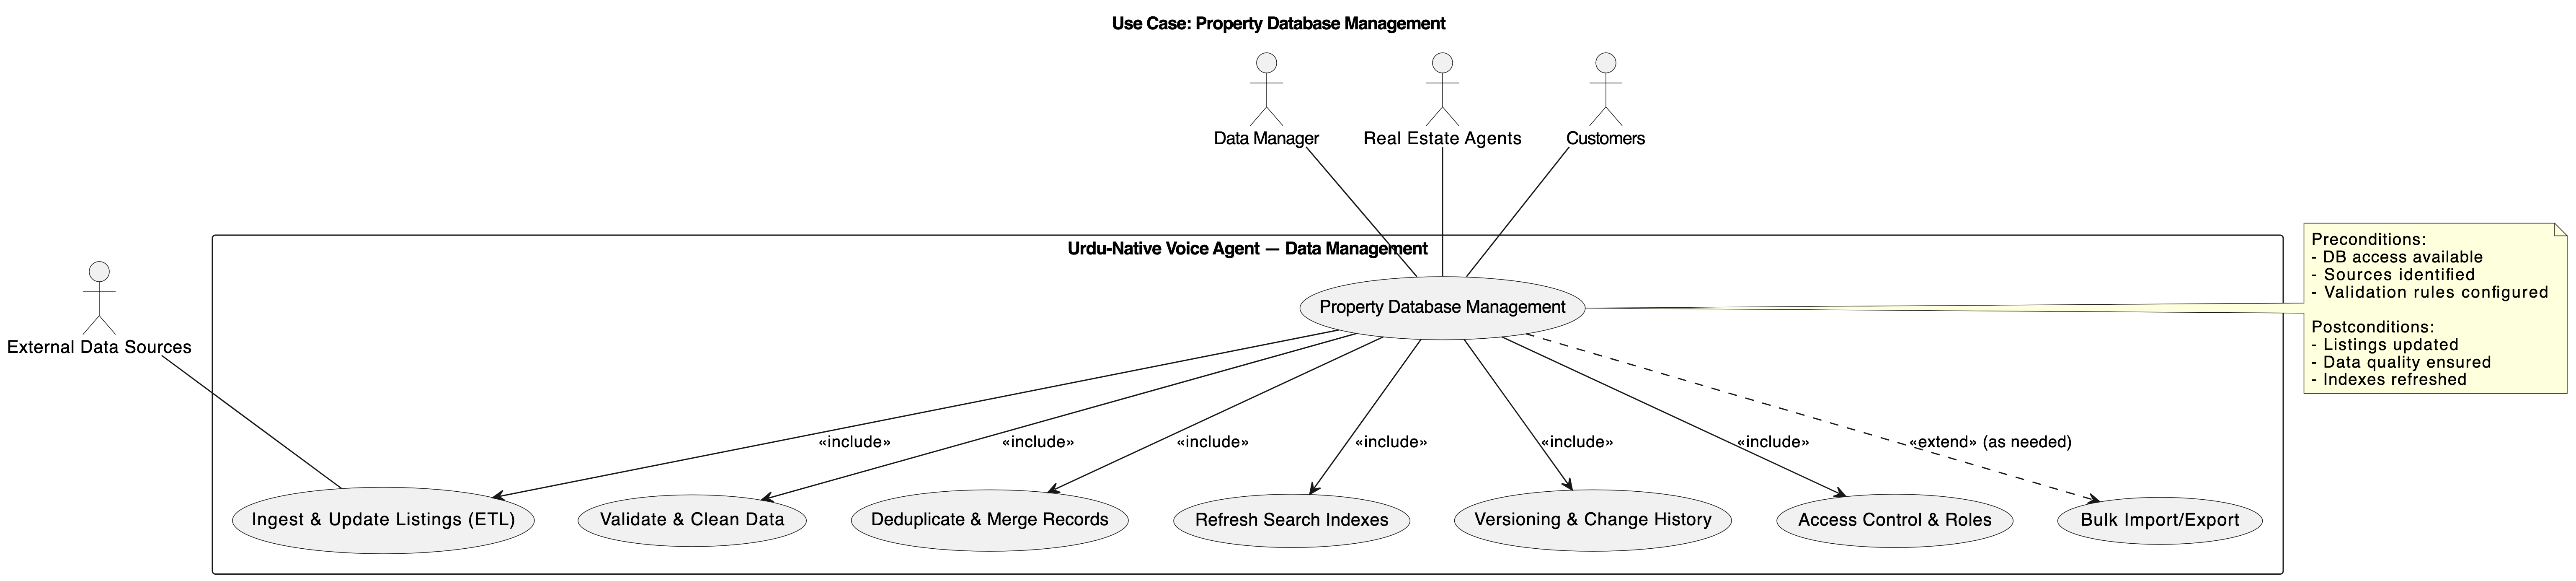
\includegraphics[width=\textwidth]{ThesisFigs/UC_Data Management.drawio}
\caption{Data Management Use Case Diagram}
\label{fig:app-uc-data}
\end{figure}

%──────────────────────────────────────────────────────────────────────────────
\section{Appendix B: Domain Model}

\begin{figure}[H]
\centering
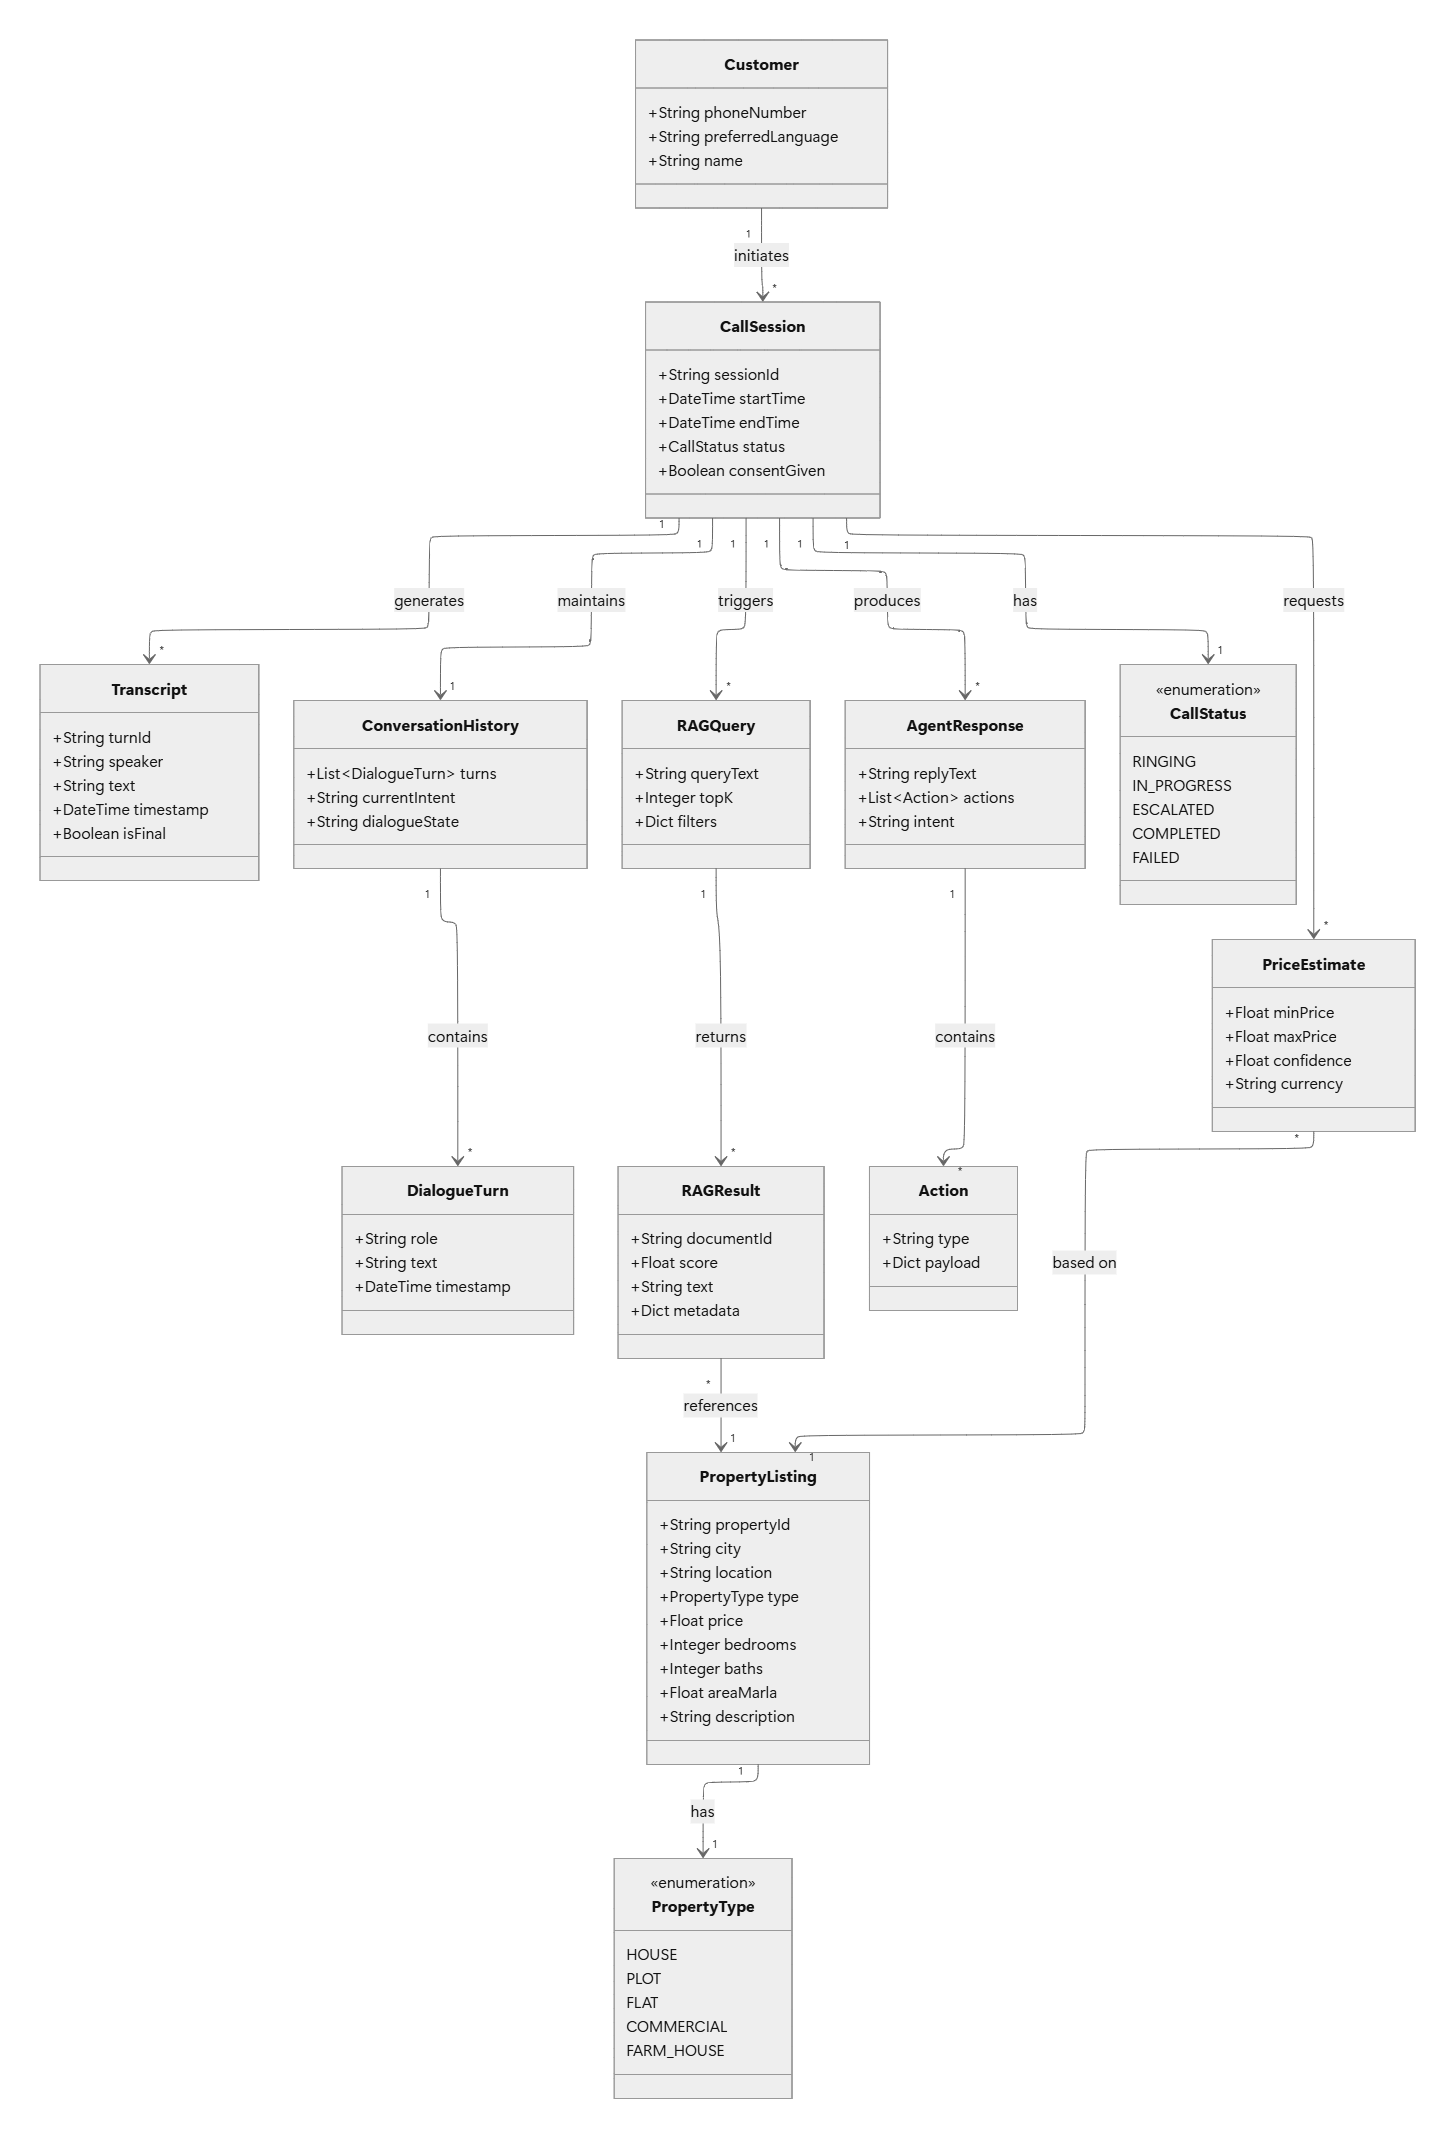
\includegraphics[width=\textwidth]{ThesisFigs/Domain Model Diagram}
\caption{ORICALO Domain Model: All Entities and Relationships}
\label{fig:app-domain-model}
\end{figure}

%──────────────────────────────────────────────────────────────────────────────
\section{Appendix C: Architecture Diagrams}

\subsection{High-Level System Architecture}
\begin{figure}[H]
\centering
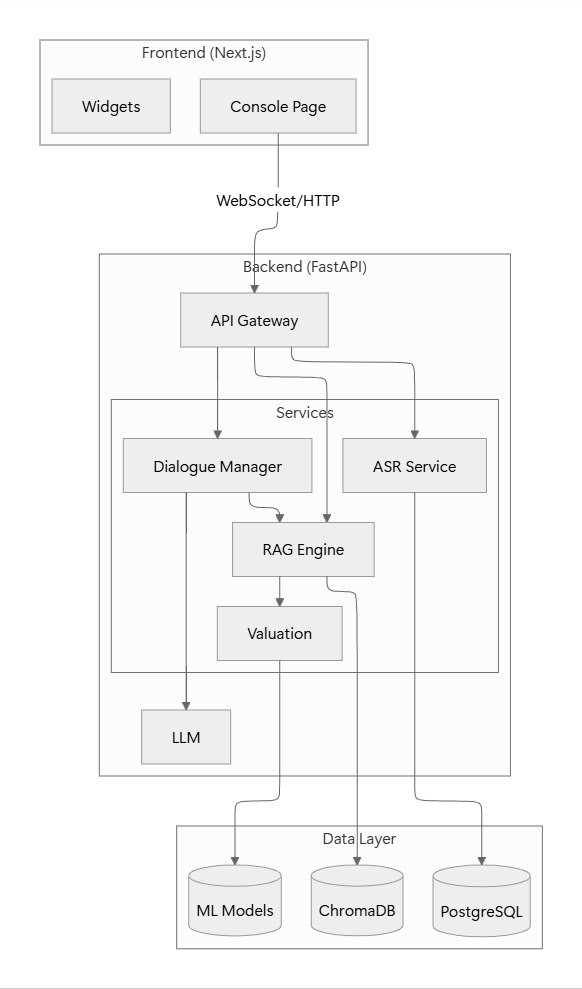
\includegraphics[width=\textwidth]{ThesisFigs/High-Level_Architecture}
\caption{ORICALO High-Level Architecture: Layered Service-Oriented Design}
\label{fig:app-hla}
\end{figure}

\subsection{RAG Pipeline Architecture}
\begin{figure}[H]
\centering
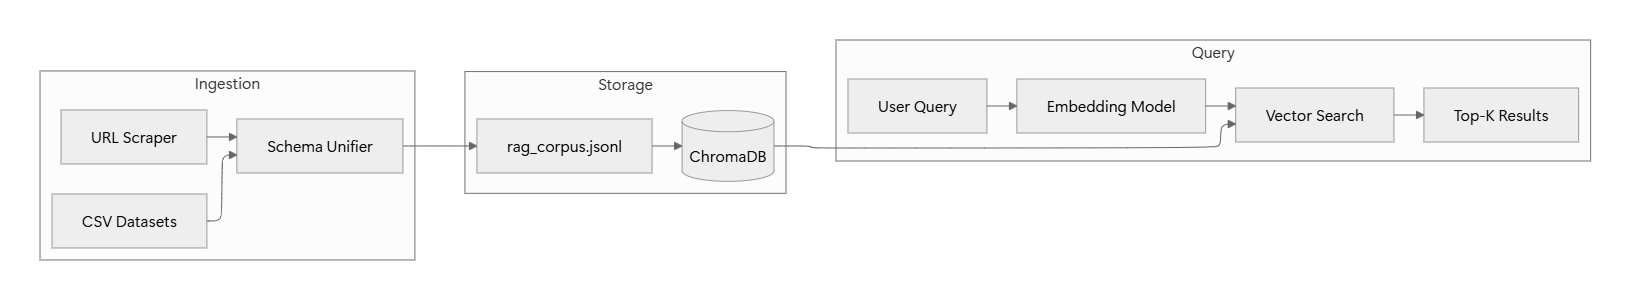
\includegraphics[width=0.85\textwidth]{ThesisFigs/RAG_Architecture}
\caption{RAG Pipeline: Data Ingestion, Vector Indexing, and Query Flow}
\label{fig:app-rag-arch}
\end{figure}

%──────────────────────────────────────────────────────────────────────────────
\section{Appendix D: Design Diagrams}

\subsection{Data Flow Diagram --- Level 0 (Context)}
\begin{figure}[H]
\centering
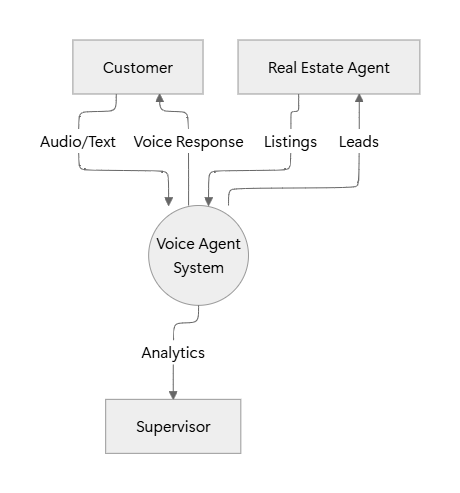
\includegraphics[width=0.75\textwidth]{ThesisFigs/Data_Flow_Diagram_Level_0}
\caption{Context-Level DFD: ORICALO System and External Entities}
\label{fig:app-dfd0}
\end{figure}

\subsection{Data Flow Diagram --- Level 1}
\begin{figure}[H]
\centering
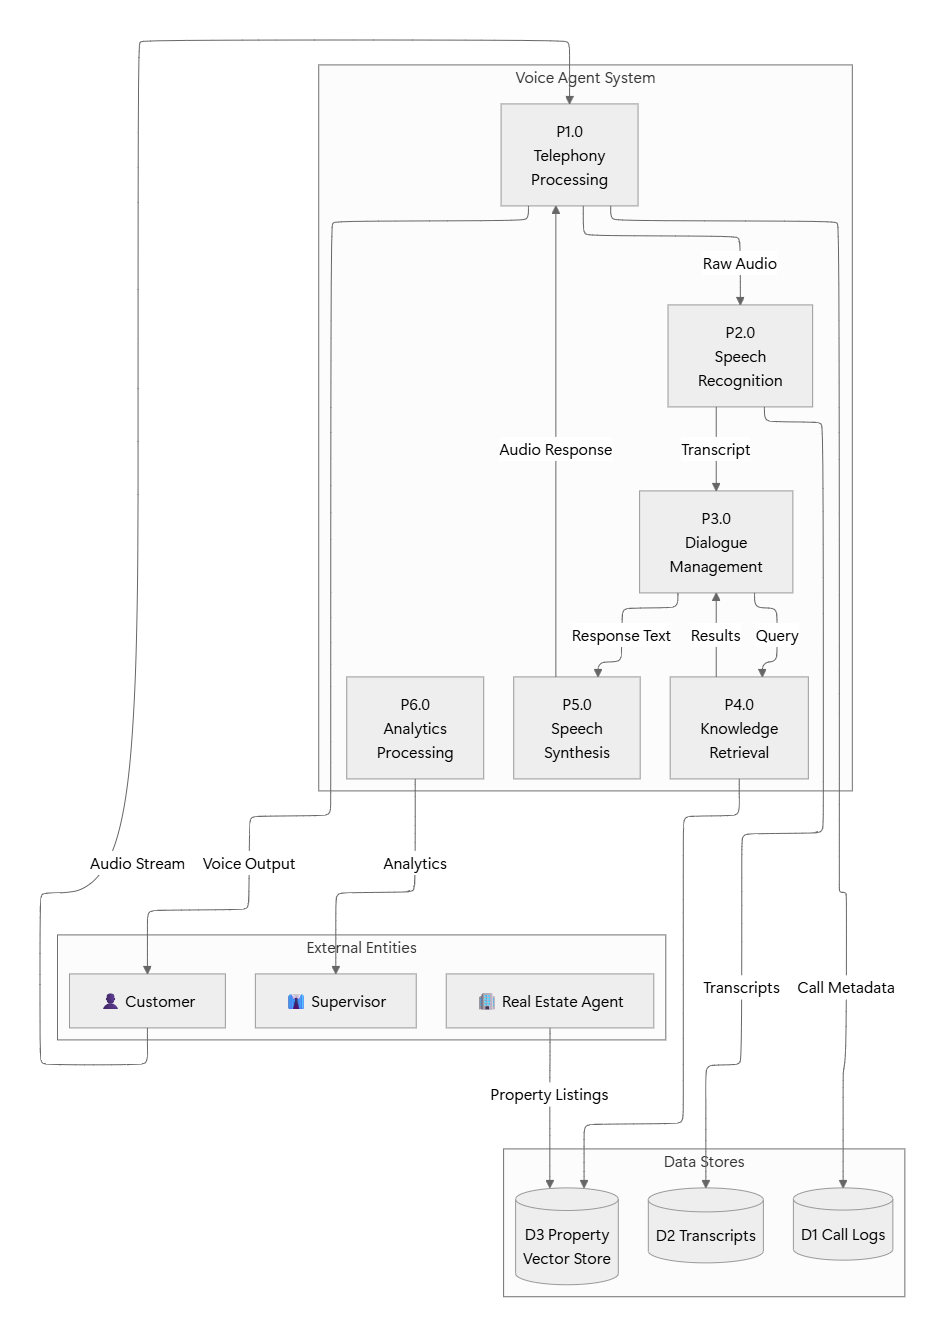
\includegraphics[width=\textwidth]{ThesisFigs/Data_Flow_Diagram_Level_1}
\caption{Level 1 DFD: Major System Processes and Data Stores}
\label{fig:app-dfd1}
\end{figure}

\subsection{Data Flow Diagram --- Level 2 (Dialogue Management)}
\begin{figure}[H]
\centering
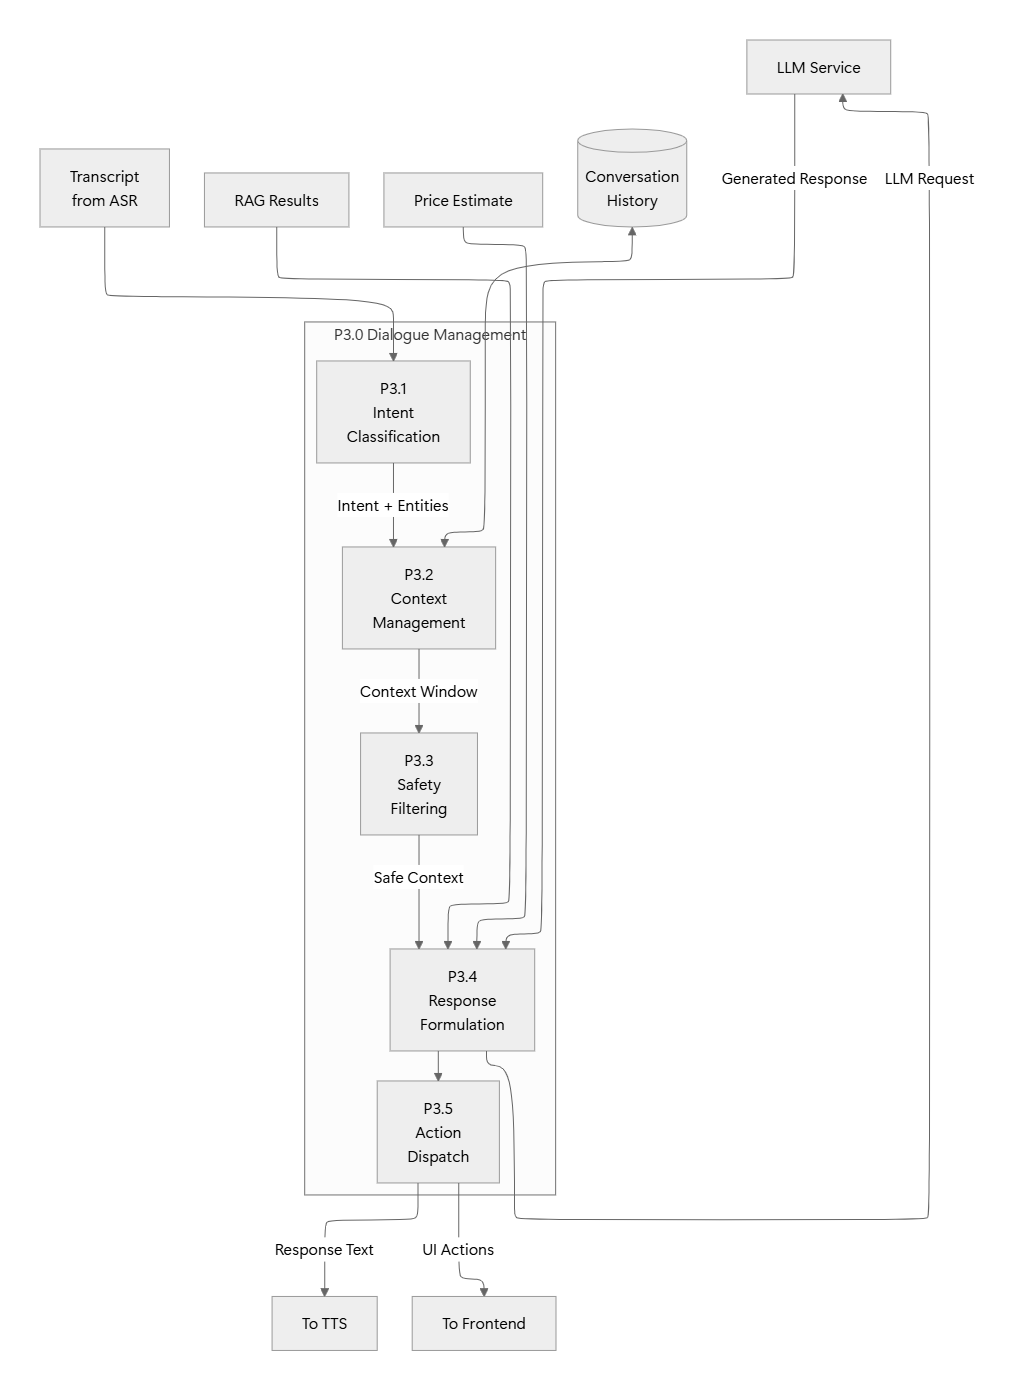
\includegraphics[width=\textwidth]{ThesisFigs/Data_Flow_Diagram_Level_2_Dialogue_Management}
\caption{Level 2 DFD: Dialogue Management Sub-Processes}
\label{fig:app-dfd2}
\end{figure}

\subsection{Sequence Diagram --- Dialogue Turn}
\begin{figure}[H]
\centering
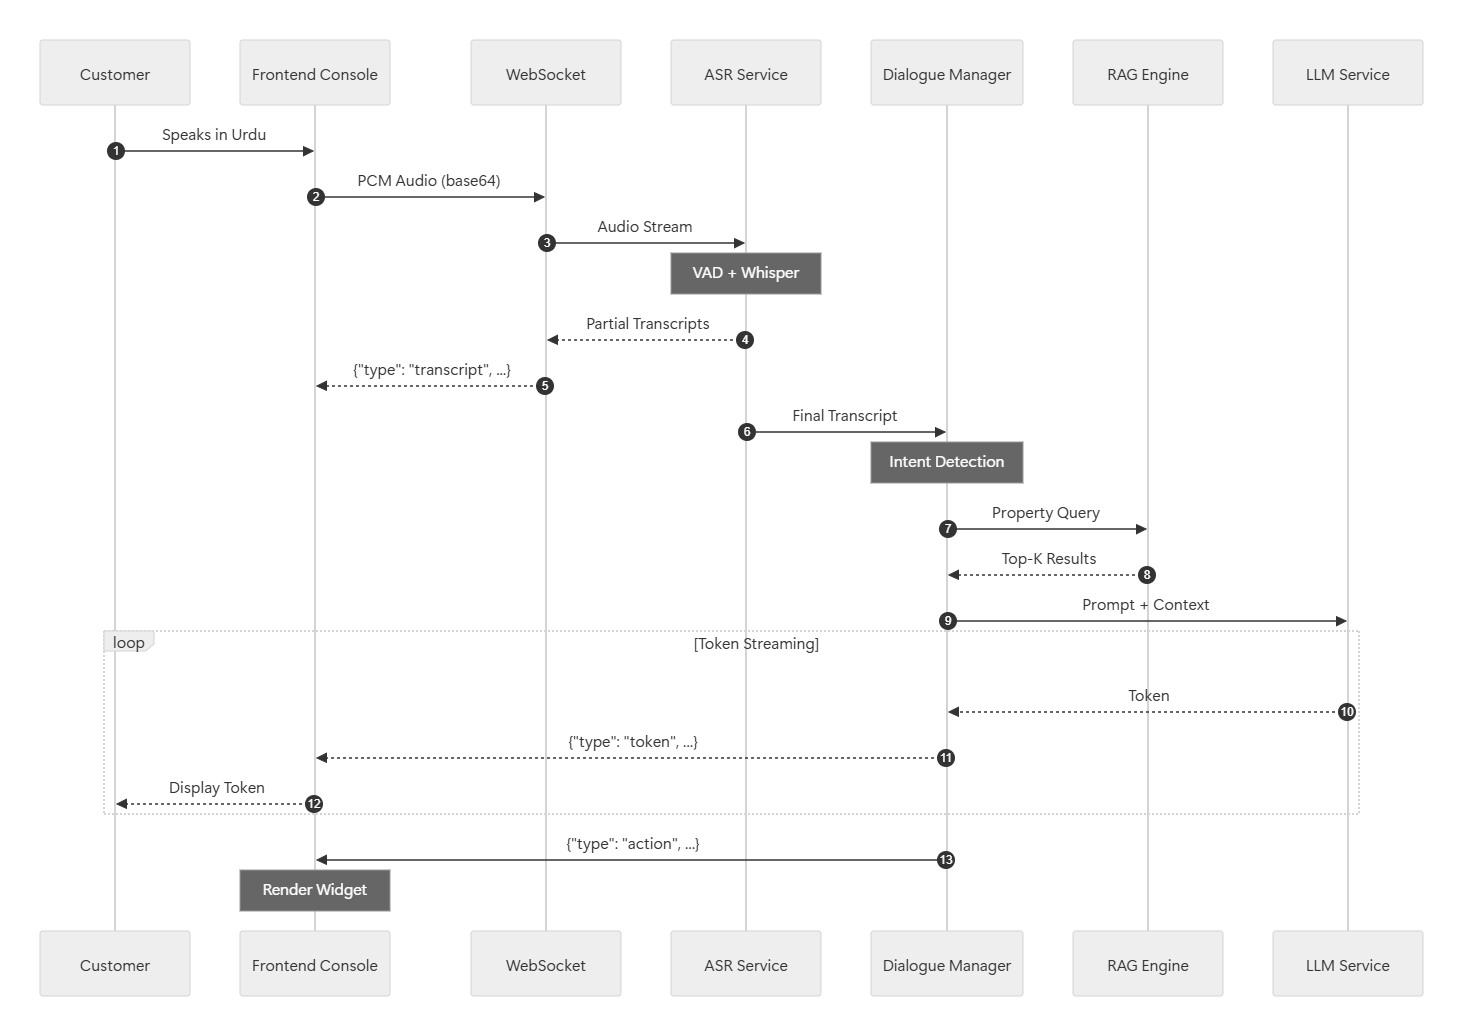
\includegraphics[width=\textwidth]{ThesisFigs/Sequence Diagram - Dialogue Turn}
\caption{Sequence Diagram: Complete Dialogue Turn with Barge-In Support}
\label{fig:app-sequence}
\end{figure}

%──────────────────────────────────────────────────────────────────────────────
\section{Appendix E: System Screenshots}

\subsection{ORICALO Console Interface}
\begin{figure}[H]
\centering
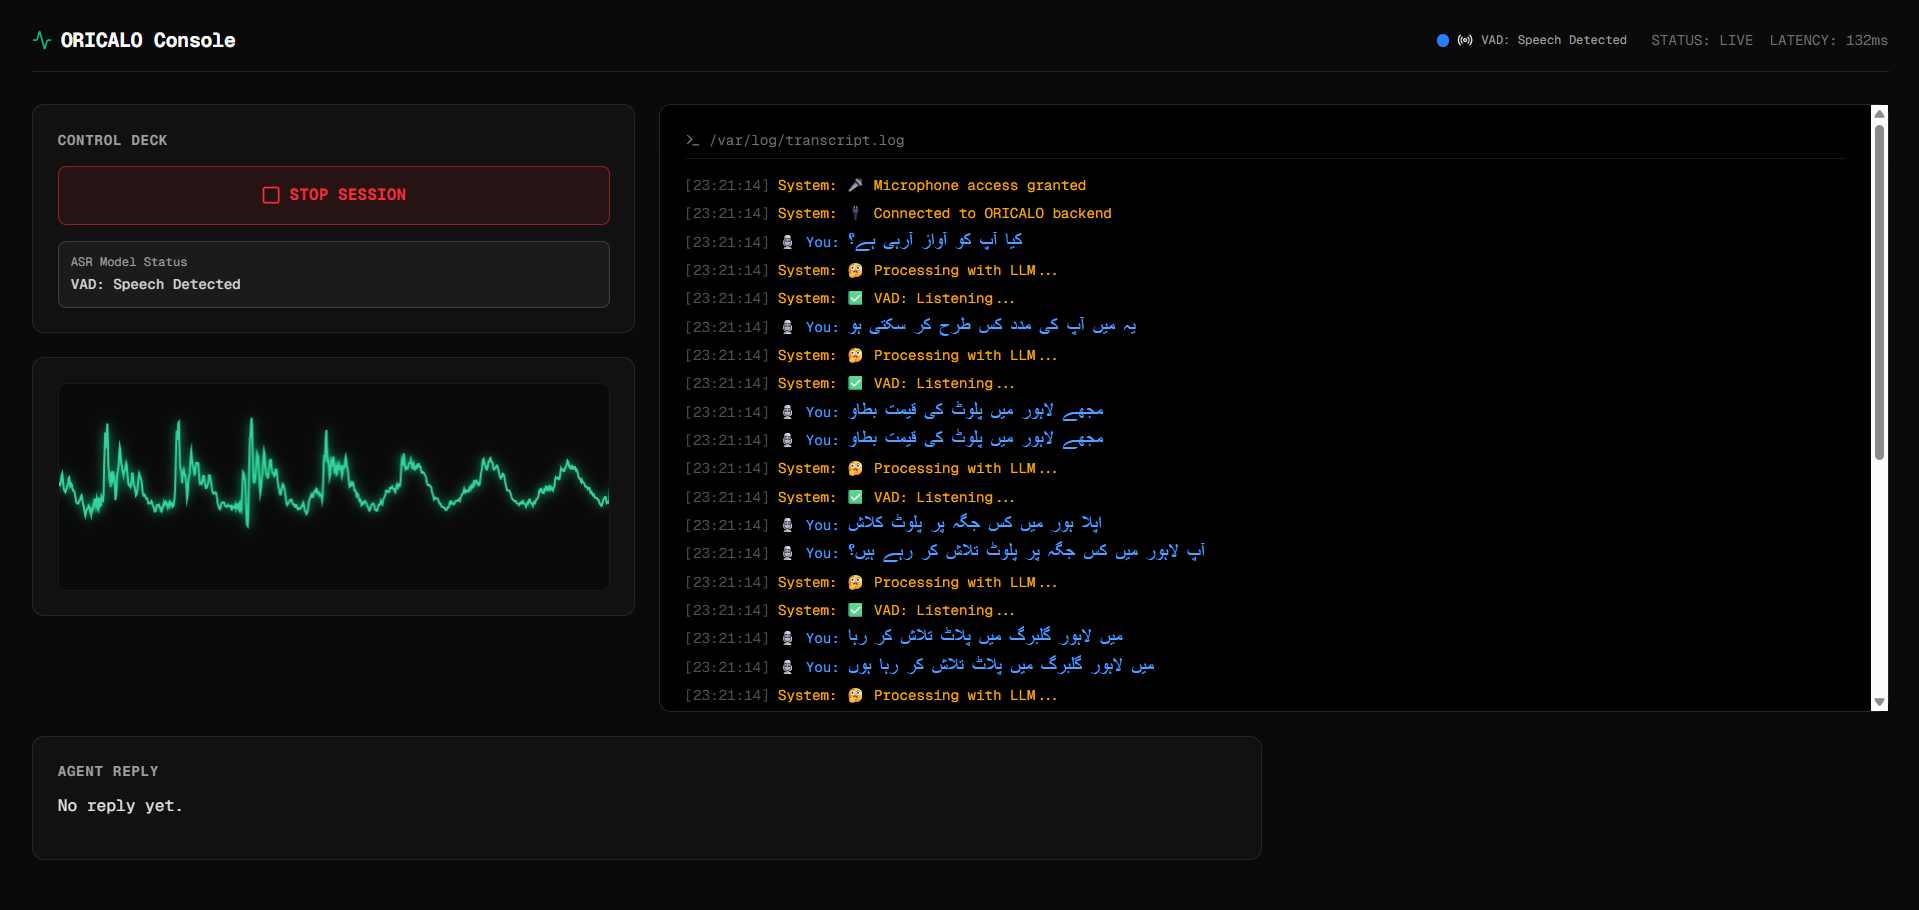
\includegraphics[width=\textwidth]{ThesisFigs/UI_screenshot}
\caption{ORICALO Voice Console: Real-Time Transcript, Waveform, and Agent Reply Panel}
\label{fig:app-ui-console}
\end{figure}

%──────────────────────────────────────────────────────────────────────────────
\section{Appendix F: Test Suite Reference}

\subsection{How to Run Tests}

\begin{enumerate}
    \item Install dependencies: \texttt{pip install -r requirements.txt}
    \item From the project root, run: \texttt{pytest tests/ -v --tb=short}
    \item For coverage: \texttt{pytest tests/ --cov=backend/app --cov-report=html}
    \item HTML coverage report opens at \texttt{htmlcov/index.html}
\end{enumerate}

\subsection{Unit Test File Reference}

\begin{table}[H]
\centering
\caption{Unit Test Files and Coverage Areas}
\renewcommand{\arraystretch}{1.2}
\begin{tabular}{|l|p{9cm}|}
\hline
\textbf{File} & \textbf{Covered Logic} \\ \hline
\texttt{test\_dialogue\_helpers.py} & \texttt{\_detect\_intent}, \texttt{\_extract\_location}, \texttt{\_get\_price\_estimate} fallback \\ \hline
\texttt{test\_valuation\_helpers.py} & \texttt{\_marla\_to\_sqft}, premium keyword detection, Pydantic schema validation \\ \hline
\texttt{test\_redact\_pii.py} & \texttt{redact\_pii} phone and CNIC pattern matching \\ \hline
\texttt{test\_voice\_orchestrator\_helpers.py} & \texttt{extract\_sentences} Urdu/English sentence buffering \\ \hline
\texttt{test\_analytics\_helpers.py} & PII edge cases, lead score boundaries, qualification labels \\ \hline
\texttt{test\_rag\_helpers.py} & Corpus schema, embedding text builder, ChromaDB filter construction \\ \hline
\texttt{test\_tts\_helpers.py} & TTS text cleaning, sentence chunking, factory backend selection \\ \hline
\end{tabular}
\label{tab:app-unit-tests}
\end{table}

\subsection{Integration Test File Reference}

\begin{table}[H]
\centering
\caption{Integration Test Files and API Coverage}
\renewcommand{\arraystretch}{1.2}
\begin{tabular}{|l|p{9cm}|}
\hline
\textbf{File} & \textbf{API Endpoints Covered} \\ \hline
\texttt{test\_health.py} & \texttt{GET /}, \texttt{GET /health} \\ \hline
\texttt{test\_agents\_api.py} & \texttt{POST /agents/}, \texttt{GET /agents/}, \texttt{GET /agents/\{id\}}, \texttt{PUT /agents/\{id\}}, \texttt{DELETE /agents/\{id\}} \\ \hline
\texttt{test\_listings\_api.py} & \texttt{POST /listings/}, \texttt{GET /listings/}, \texttt{GET /listings/\{id\}}, \texttt{PUT /listings/\{id\}}, \texttt{DELETE /listings/\{id\}} \\ \hline
\texttt{test\_valuation\_api.py} & \texttt{POST /valuation/predict}, \texttt{GET /valuation/stats} \\ \hline
\texttt{test\_crm\_api.py} & \texttt{POST/GET/PUT/DELETE /crm/leads}, \texttt{GET /crm/sessions}, \texttt{GET /crm/action\_items} \\ \hline
\end{tabular}
\label{tab:app-integration-tests}
\end{table}